
\subsection{Conception de la commande de l'axe motorisé d'élévation à partir
des performances attendues et vérification des performances
simulées du FLIR}

\begin{obj}
Modéliser l'asservissement de l'axe motorisé d'élévation, concevoir sa commande puis vérifier ses performances
simulées vis-à-vis du cahier des charges donné sur le tableau \ref{tab2}.
\end{obj}

\begin{table}[!htb]
\begin{center}
\begin{tabular}{|p{0.3\textwidth}|p{0.3\textwidth}|p{0.3\textwidth}|}
\hline 
\textbf{Exigence} & \textbf{Critère} & \textbf{Valeur} \\ 
\hline 
1.4 Acquérir une image du paysage
extérieur suivant la ligne de visée
du pilote & Retard de trainage maximal de la
ligne de visée du FLIR & $40ms$ \\ 
\cline{2-3} 
& Précision angulaire de la ligne de
visée du FLIR & $680\mu rad$\\ 
\cline{2-3}  
 & Stabilité de la ligne de visée du
FLIR & Oscillations d'amplitude inférieure
à $340 \mu rad$ \\ 
\hline  
Être insensible aux perturbations
de l'air ambiant & Forme extérieure & Couple aérodynamique minimum\\ 
\hline
\end{tabular} 
\caption{Cahier des charges partiel du FLIR \label{tab2}}
\end{center}
\end{table}

%\FloatBarrier
\subsubsection{Modélisation de l'asservissement de l'étage fin d'élévation}

\begin{obj}
En s'appuyant sur les hypothèses validées en partie \ref{partie2}, compléter la modélisation de l'asservissement de
l'étage fin d'élévation et ajuster un correcteur qui lui permette d'atteindre les performances attendues.
\end{obj}

Un gyromètre est placé directement sur l'étage fin d'élévation et permet de mesurer $\omega_{fe0\text{ mes}}(t)$, taux de rotation de l'étage fin d'élévation par rapport au référentiel galiléen $R_0$. Les ingénieurs ont donc choisi d'asservir l'étage
fin d'élévation en vitesse angulaire afin d'utiliser directement la mesure du gyromètre.

La direction de la ligne de visée est paramétrée par rapport au référentiel galiléen $R_0$ par l'angle $\theta_{fe0}(t)=\theta_{e0}(t)$.

Sont donnés les éléments suivants :
\begin{itemize}
\item $\dot{\theta}_{fe0}(t)=\omega_{fe0}(t)=\vect{\Omega}(fe/R_0)\cdot \vect{y}_e$ où $\vect{\Omega}(fe/R_0)$ est le vecteur taux de rotation de l'étage fin d'élévation ($fe$) dans
son mouvement par rapport au référentiel terrestre $R_0$ ;
\item le comportement du gyromètre, placé directement sur l'étage fin d'élévation, peut être modélisé par un
premier ordre de gain unitaire et de bande passante à $-3 dB$ égale à $100 Hz$ ;
\item l'étage fin d'élévation ($f_e$) est actionné par un moteur électrique linéaire comme indiqué sur la figure\ref{figure14},
dont la tige est en liaison sphérique en $A$ avec l'étage fin d'élévation et le carter en liaison sphérique en $B$ avec l'étage gros d'élévation ;
\item l'isolement de la tige seule du moteur électrique linéaire permet de modéliser son action mécanique de liaison
en $A$ sur l'étage fin d'élévation par un glisseur au point $A$ de résultante $F_{mot}(t)\vect{u}$ ;
\item l'étage fin d'élévation ($fe$) est en liaison pivot d'axe $\axe{P}{\vect{y_e}}$ avec l'étage gros d'élévation ($ge$) ;
\item $\vect{AP}=r\cdot \vect{x}_e$ avec $r=10cm$ ;
\item $\lambda(t)$ paramètre la position de la tige par rapport au carter du moteur électrique linéaire tel que $\vect{BA}=\lambda(t)\cdot \vect{u}$.
\end{itemize}

Le choix de la motorisation de l'étage fin d'élévation permet d'atteindre des accélérations importantes mais
l'amplitude du mouvement de l'étage fin d'élévation ($fe$) par rapport à l'étage gros d'élévation ($ge$) est limitée
à l'intervalle $\left[-5^{\circ}, +5^{\circ}\right]$. Il est donc nécessaire d'orienter également l'étage gros d'élévation ($ge$) grâce au moteur à courant continu de la figure \ref{figure14}.

Hypothèses :
\begin{itemize}
\item le porteur est en translation suivant $\vect{z}_0$ par rapport au référentiel galiléen $R_0$ ;
\item l'étage gros d'élévation ($ge$) est fixe par rapport au porteur, c'est-à-dire que $\dot{\theta}_{ge0}(t)=\omega_{ge0}(t)=0$ et
$\theta_{ge0}(t) = a$, avec $a$ un angle constant ;
\item l'orientation de l'étage gros d'élévation ($ge$) est telle que $\vect{u}\approx \vect{z}_e$ ;
\item la liaison pivot entre l'étage fin d'élévation ($fe$) et l'étage gros d'élévation ($ge$) est parfaite ;
\item le moment d'inertie de l'étage fin d'élévation ($fe$) autour de l'axe $\axe{P}{\vect{y_e}}$ est noté $B_{fe}=0,1kg\cdot m^2$ ;
\item le centre de gravité de l'étage fin d'élévation ($fe$) est considéré en $P$ , c'est-à-dire que $P=G_{fe}$ (voir figure 12) ;
\item $\vect{V}(A\in fe/ge)=v_{tige}(t)\cdot \vect{z}_e$ avec $\dot{\lambda}(t)=v_{tige}(t)$ et $\vect{u}\approx \vect{z}_e$ ;
\item $\vect{V}(A\in ge/R_0)=\vect{V}(P\in ge/R_0)=v(t)\cdot \vect{z}_0$ .
\end{itemize}


\begin{figure}[!htb]
\begin{center}
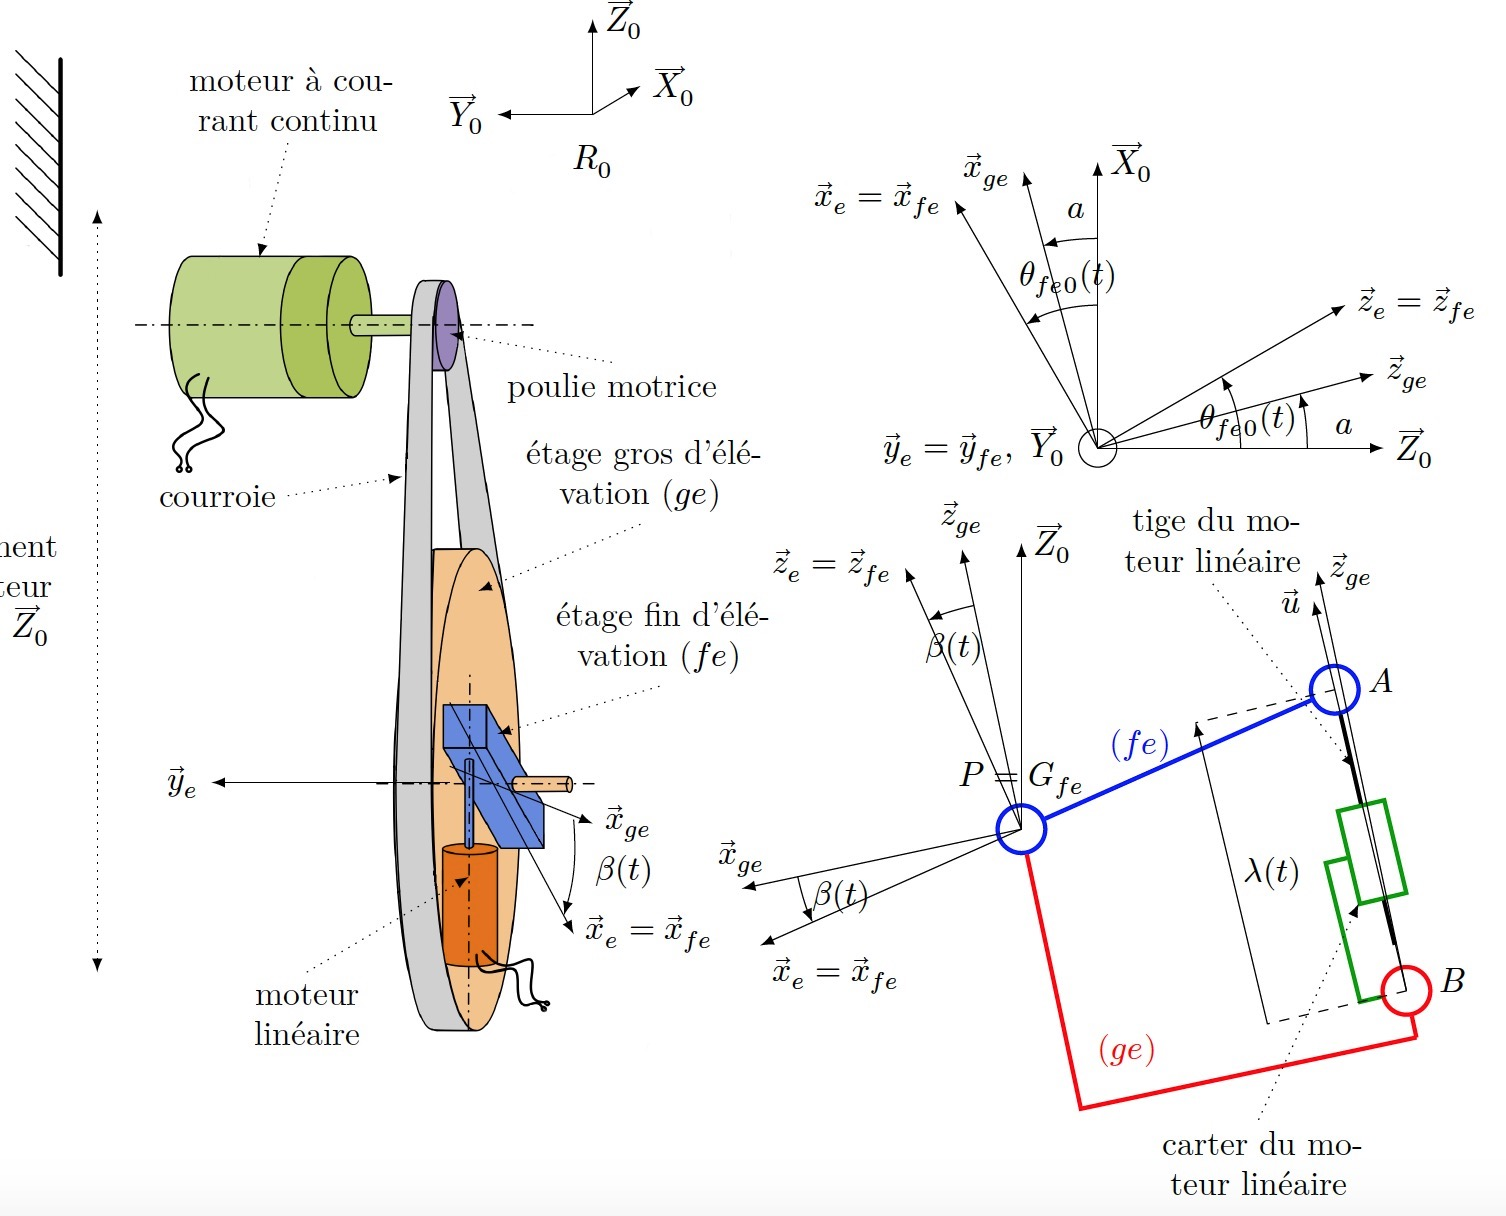
\includegraphics[width=0.9\textwidth]{figure14.jpg}
\caption{Structure et paramétrage des étages fin et gros de l'axe motorisé d'élévation \label{figure14}}
\end{center}
\end{figure}

\question{Exprimer le vecteur vitesse $\vect{V}(A\in fe/R_0)$ en fonction de $r$, $v(t)$ et $\dot{\theta}_{fe0}(t)$, puis en déduire une relation entre $v_{tige}(t)$ et $\dot{\theta}_{fe0}(t)$.}

Dans la suite du sujet, le passage dans le domaine symbolique de Laplace est noté de la façon suivante : $F(p)$
est la transformée de Laplace de la fonction $f(t)$, avec $p$ la variable de Laplace. Les conditions de Heaviside sont
vérifiées, c'est-à-dire que les valeurs initiales des fonctions temporelles sont nulles.

\question{En appliquant le théorème du moment dynamique à l'étage fin d'élévation ($fe$), exprimer littéralement la
fonction de transfert $\dfrac{\Omega_{fe0}(p)}{F_{mot}(p)}$ de la figure \ref{figure15} et en déduire les expressions de $M_{eq}$ et $K_1$. Effectuer les applications numériques.}

On rappelle que le gyromètre, placé directement sur l'étage fin d'élévation, permet de mesurer $\omega_{fe0\text{ mes}}(t)$. Son comportement peut être modélisé par un premier ordre de la forme $\dfrac{1}{1+\tau_{gyro}p}$ et de bande passante à $-3 dB$ égale à $100 Hz$.



\question{Calculer la valeur numérique de $\tau_{gyro}$.}

Le modèle d'asservissement de l'étage fin d'élévation étant établi, il est alors possible de concevoir sa commande.

%\FloatBarrier
\subsubsection{Conception de la commande de l'étage fin d'élévation}

Les performances de l'étage fin d'élévation ont été déterminées à partir des performances du FLIR établies en
partie \ref{partie1}. Elles sont données dans le tableau de la figure \ref{figure15}.

La consigne de vitesse $\dot{\theta}_{fe0\text{cons}}=\omega_{fe0\text{cons}}(t)$ est établie par rapport au référentiel galiléen $R_0$. Elle est calculée à partir de la détection de posture (DDP du casque TopOwl) de la tête du pilote et des informations
d'orientation du porteur par rapport au référentiel terrestre $R_0$ obtenues par la centrale inertielle du porteur.

\begin{figure}[!htb]
\begin{center}
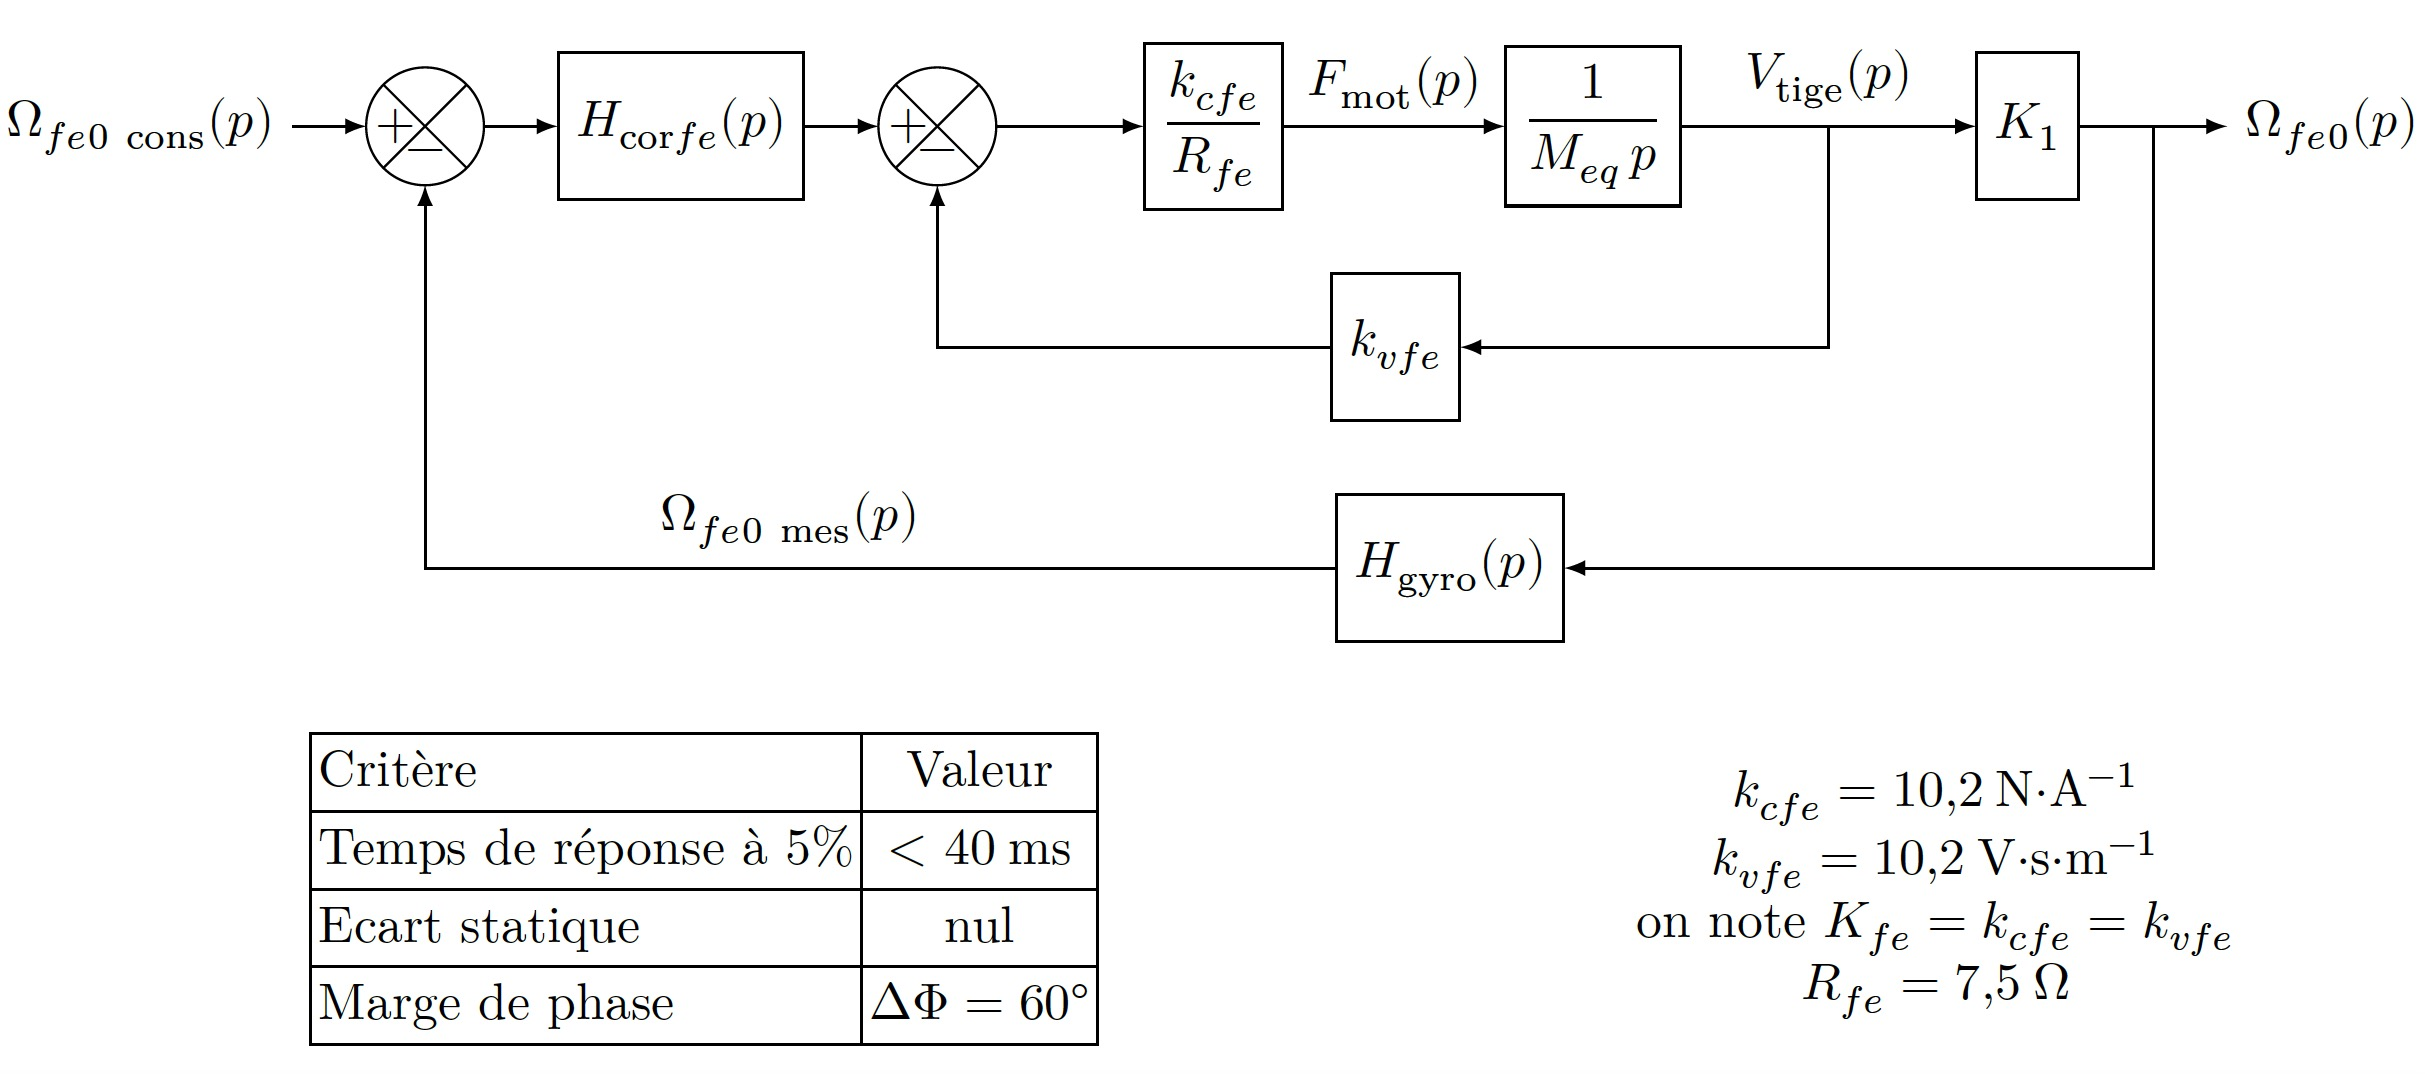
\includegraphics[width=0.9\textwidth]{figure15.jpg}
\caption{Modèle d'asservissement de l'étage fin d'élévation et performances attendues \label{figure15}}
\end{center}
\end{figure}

Dans un premier temps, l'asservissement de vitesse n'est pas corrigé, c'est-à-dire que $H_{corfe}(p)=1$.

\question{Exprimer littéralement et sous forme canonique la fonction de transfert $H_{fe1}(p)=\dfrac{\Omega_{fe0}(p)}{\Omega_{fe0cons}(p)}$, en fonction de $K_1$, $\tau_{gyro}$, $M_{eq}$, $K_{fe}$ et $R_{fe}$.}

Compte tenu des temps de réponse à observer, on montre que $H_{fe1}(p)$ peut se mettre sous la forme simplifiée
suivante :

\begin{align*}
H_{fe1}(p)\approx\dfrac{0,5}{1+3,65\times 10^{-1}p+6\times 10^{-4}p^2}
\end{align*}

\question{En utilisant l'abaque de la figure \ref{fig16}, déterminer le temps de réponse à $5\%$ et l'écart statique de
l'asservissement en vitesse de l'étage fin d'élévation en réponse à un échelon de vitesse unitaire. Conclure sur le
respect des performances en rapidité et en précision données sur la figure \ref{fig16}.}

\begin{figure}[!htb]
\begin{center}
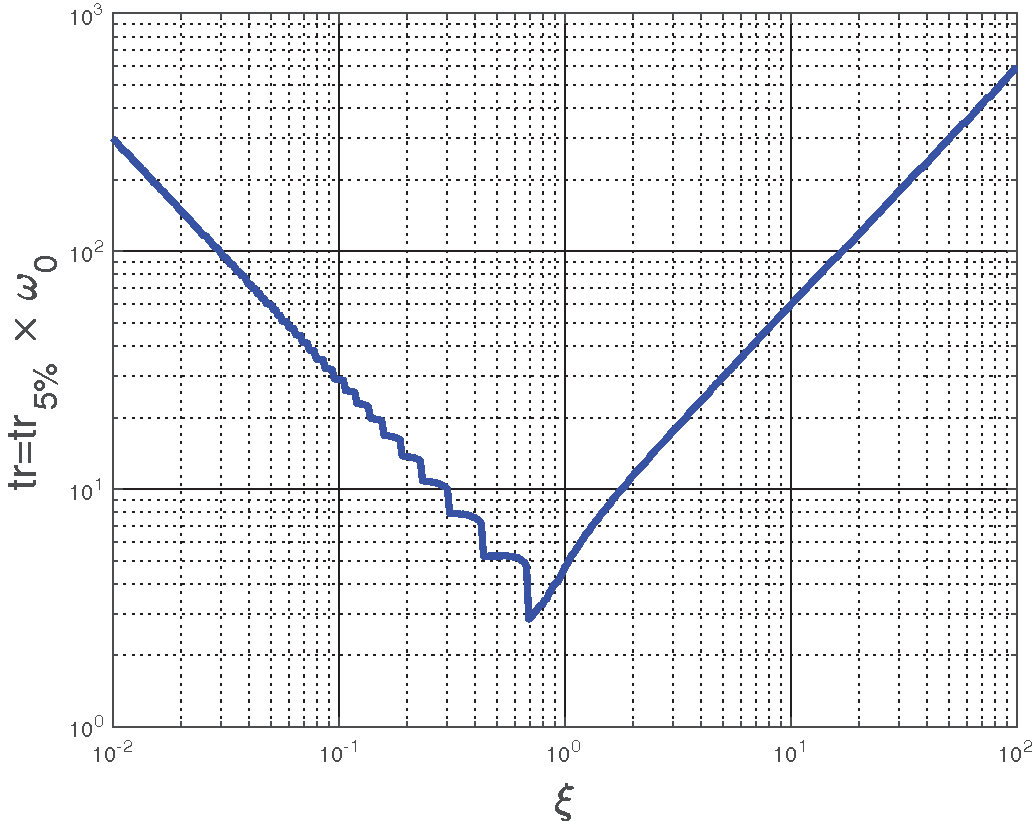
\includegraphics[width=0.6\textwidth]{amortissement.pdf}
\caption{Abaque des temps de réponse réduit\label{fig16}}
\end{center}
\end{figure}

On propose d'utiliser un correcteur proportionnel intégral de la forme $H_{corfe}(p) = K_{pfe}\left(1+\frac{1}{T_{ife}p}\right)$. La
fonction de transfert en boucle ouverte de l'asservissement en vitesse de l'étage fin d'élévation devient alors

\begin{align*}
H_{BOfe}(p)=K_{pfe}\left(1+\frac{1}{T_{ife}p}\right)\dfrac{1}{1+0,75p}\dfrac{1}{1+1,6\times 10^{-3}p}
\end{align*}

La figure \ref{figdr} du document réponse correspond aux tracés des diagrammes de Bode réels de $H_{BOfe}(j\omega)$ pour
$K_{pfe}=1$ et $T_{ife}= 0,1 s$, puis $T_{ife} = 0,01 s$.

\question{Sur cette même figure du document réponse, tracer le diagramme de phase asymptotique de $H_{BOfe}(j\omega)$
(Bode) pour $T_{ife}=0,1s$, en indiquant la pulsation $1/T_{ife}$.}



La lecture du tracé réel de la phase met en évidence un maximum à la pulsation $\omega_{max}$ telle que $\omega_{max}\in
\left[\dfrac{1}{T_{ife}}; 600\right] rad\cdot s^{-1}$.

\question{En supposant que le tracé réel semi-logarithmique de la phase est symétrique autour de $\omega_{max}$, calculer
la valeur de $T_{ife}$ comprise dans la décade $\left[0,01 s; 0,1 s\right]$ qui permet de régler ce maximum à $-120^{\circ}$.}


\question{Pour le réglage de $T_{ife}$ calculé à la question précédente avec $K_{pfe}=1$ et à partir des tracés réels du document réponse, calculer la valeur de $K_{pfe}$ qui permet de respecter le critère de marge de phase du tableau de la figure \ref{figure15}.}

Le modèle est complété en utilisant les réglages déterminés aux deux questions précédentes pour $K_{pfe}$ et $T_{ife}$. Afin de prendre en compte les caractéristiques du moteur linéaire, une saturation d'alimentation du moteur à 24 V est
ajoutée ainsi qu'une modification de la commande associée qui n'est pas étudiée ici et qui ne modifie pas les
réglages de $K_{pfe}$ et $T_{ife}$ déterminés précédemment. La réponse simulée $\omega_{fe0}(t)$ de l'étage fin d'élévation à une consigne de vitesse en échelon $\omega_{fe0cons}(t) = 1 rad\cdot s^{-1}$ est donnée sur la figure \ref{fig17}.

\begin{figure}[!htb]
\begin{center}
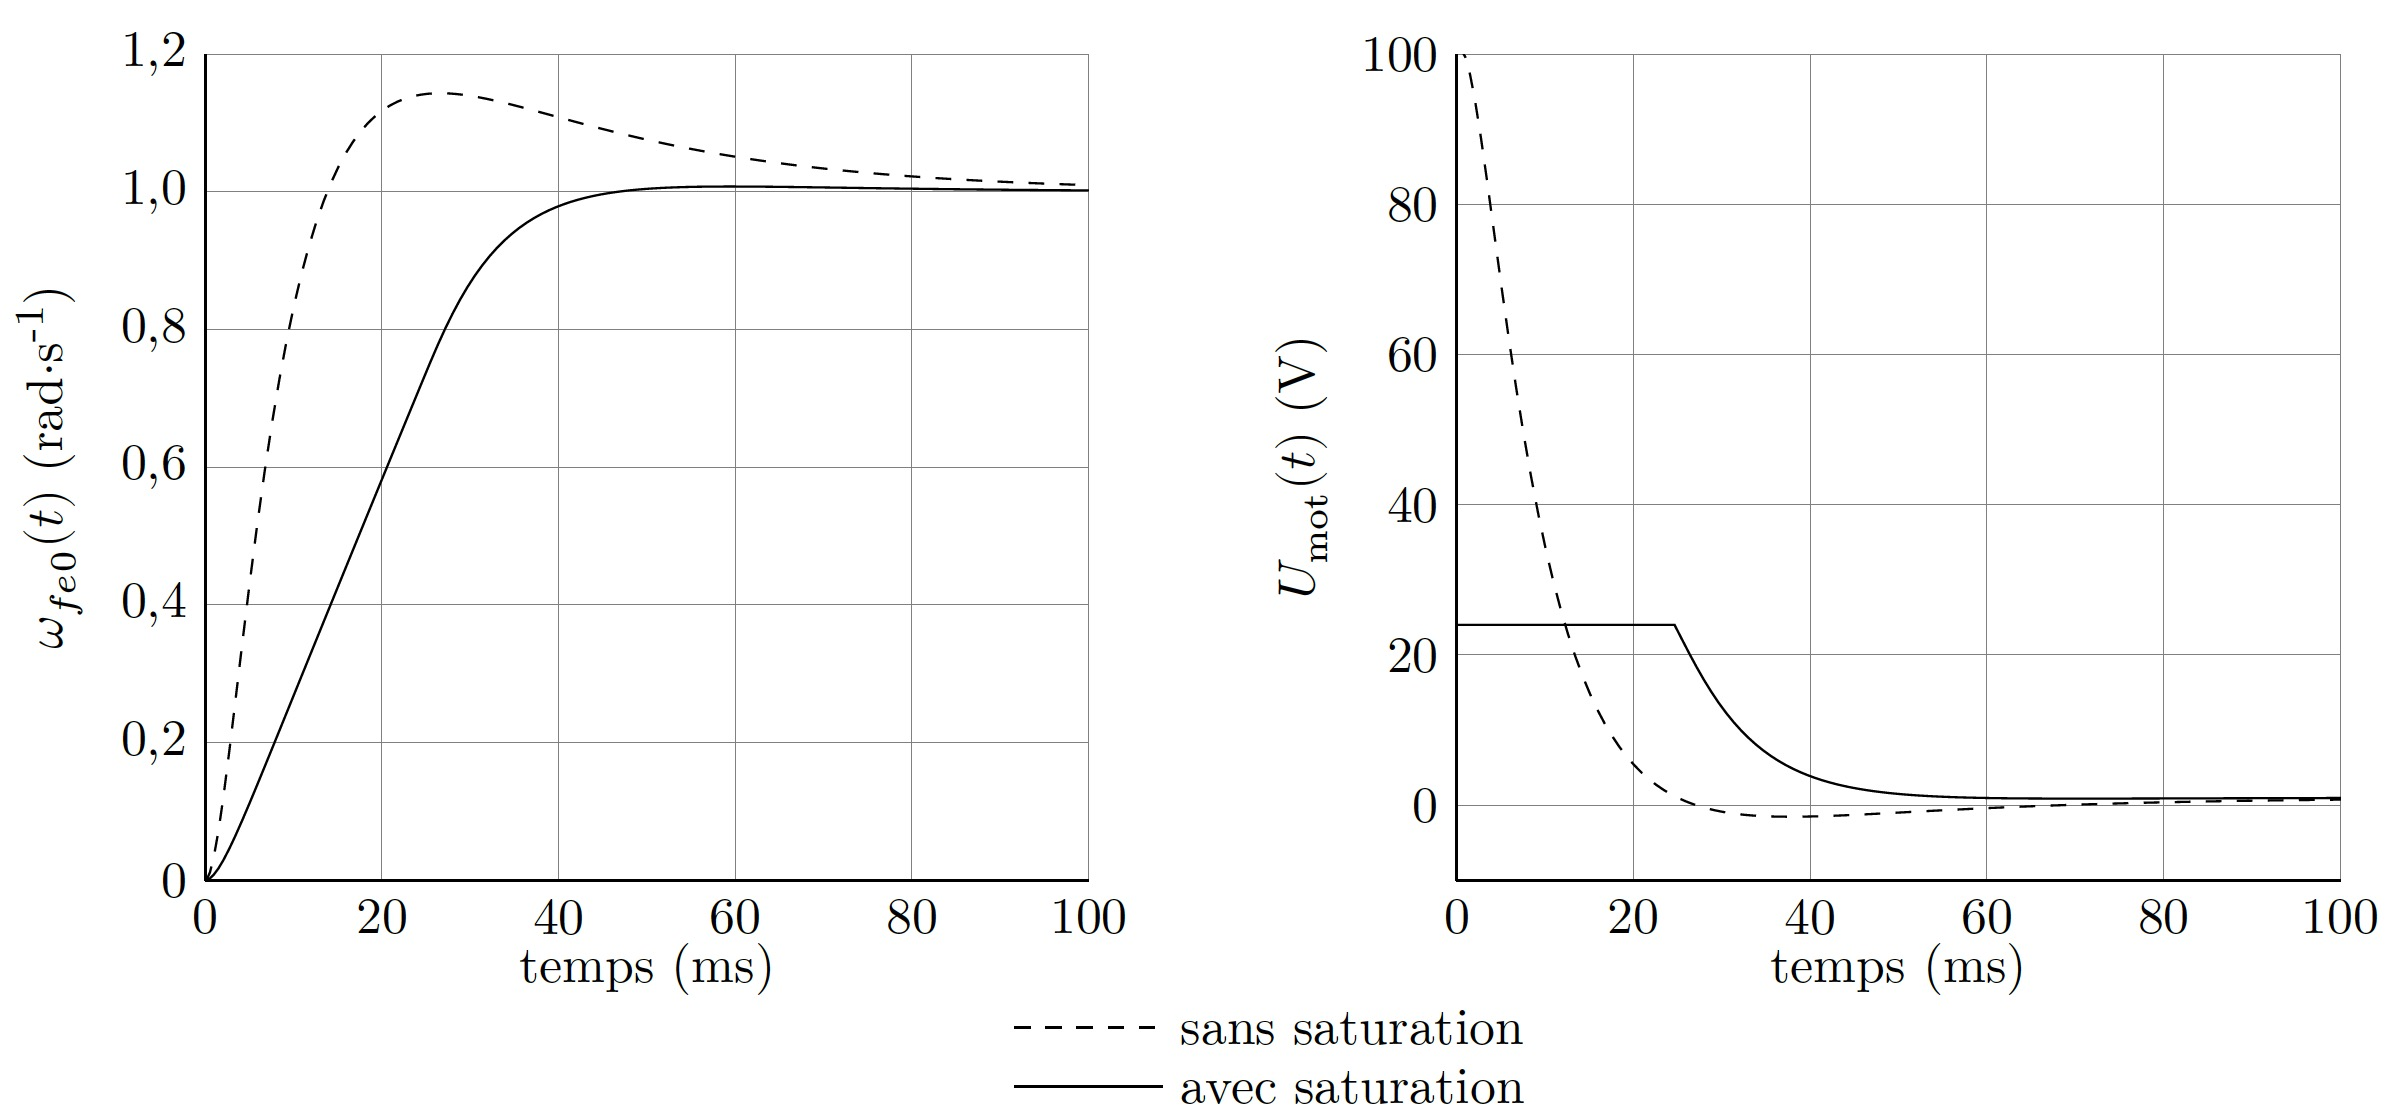
\includegraphics[width=1.0\textwidth]{figure17.jpg}
\caption{$\omega_{fe0}(t)$ et $U_{mot}(t)$ en fonction du temps avec et sans saturation de l'alimentation du moteur\label{fig17}}
\end{center}
\end{figure}

\question{D'après la figure \ref{fig17}, définir le temps pendant lequel la tension du moteur linéaire a été saturée et
expliquer les effets de cette saturation sur les performances simulées par rapport aux performances simulées
en gardant le modèle linéaire. Conclure sur la pertinence de la prise en compte de la saturation et sur les
performances de l'étage fin d'élévation.}

%\FloatBarrier
\subsubsection{Synthèse : validation des performances simulées du FLIR}

\begin{obj}
Simuler le comportement de l'axe motorisé d'élévation du FLIR et vérifier s'il respecte le cahier des
charges donné sur le tableau \ref{tab2}.
\end{obj}

À l'instar de l'étage fin d'élévation, l'étage gros d'élévation est également asservi, mais en position angulaire. Il
doit permettre à l'étage fin d'élévation de vérifier l'hypothèse émise précédemment, soit $\vect{u}\approx \vect{z}_e$, c'est-à-dire que l'angle $\beta(t)$ doit rester dans l'intervalle $\left[-5^{\circ}, +5^{\circ}\right]$.

Un capteur LVDT (Linear Variable Differential Transformer) permet de mesurer l'écart entre l'orientation de
l'étage fin d'élévation et l'étage gros d'élévation $\beta(t)=\theta_{fe0(t)}-\theta_{ge0}(t)$. Le modèle d'asservissement de l'axe
motorisé d'élévation est alors celui donné sur la figure \ref{fig18}.


\begin{figure}[!htb]
\begin{center}
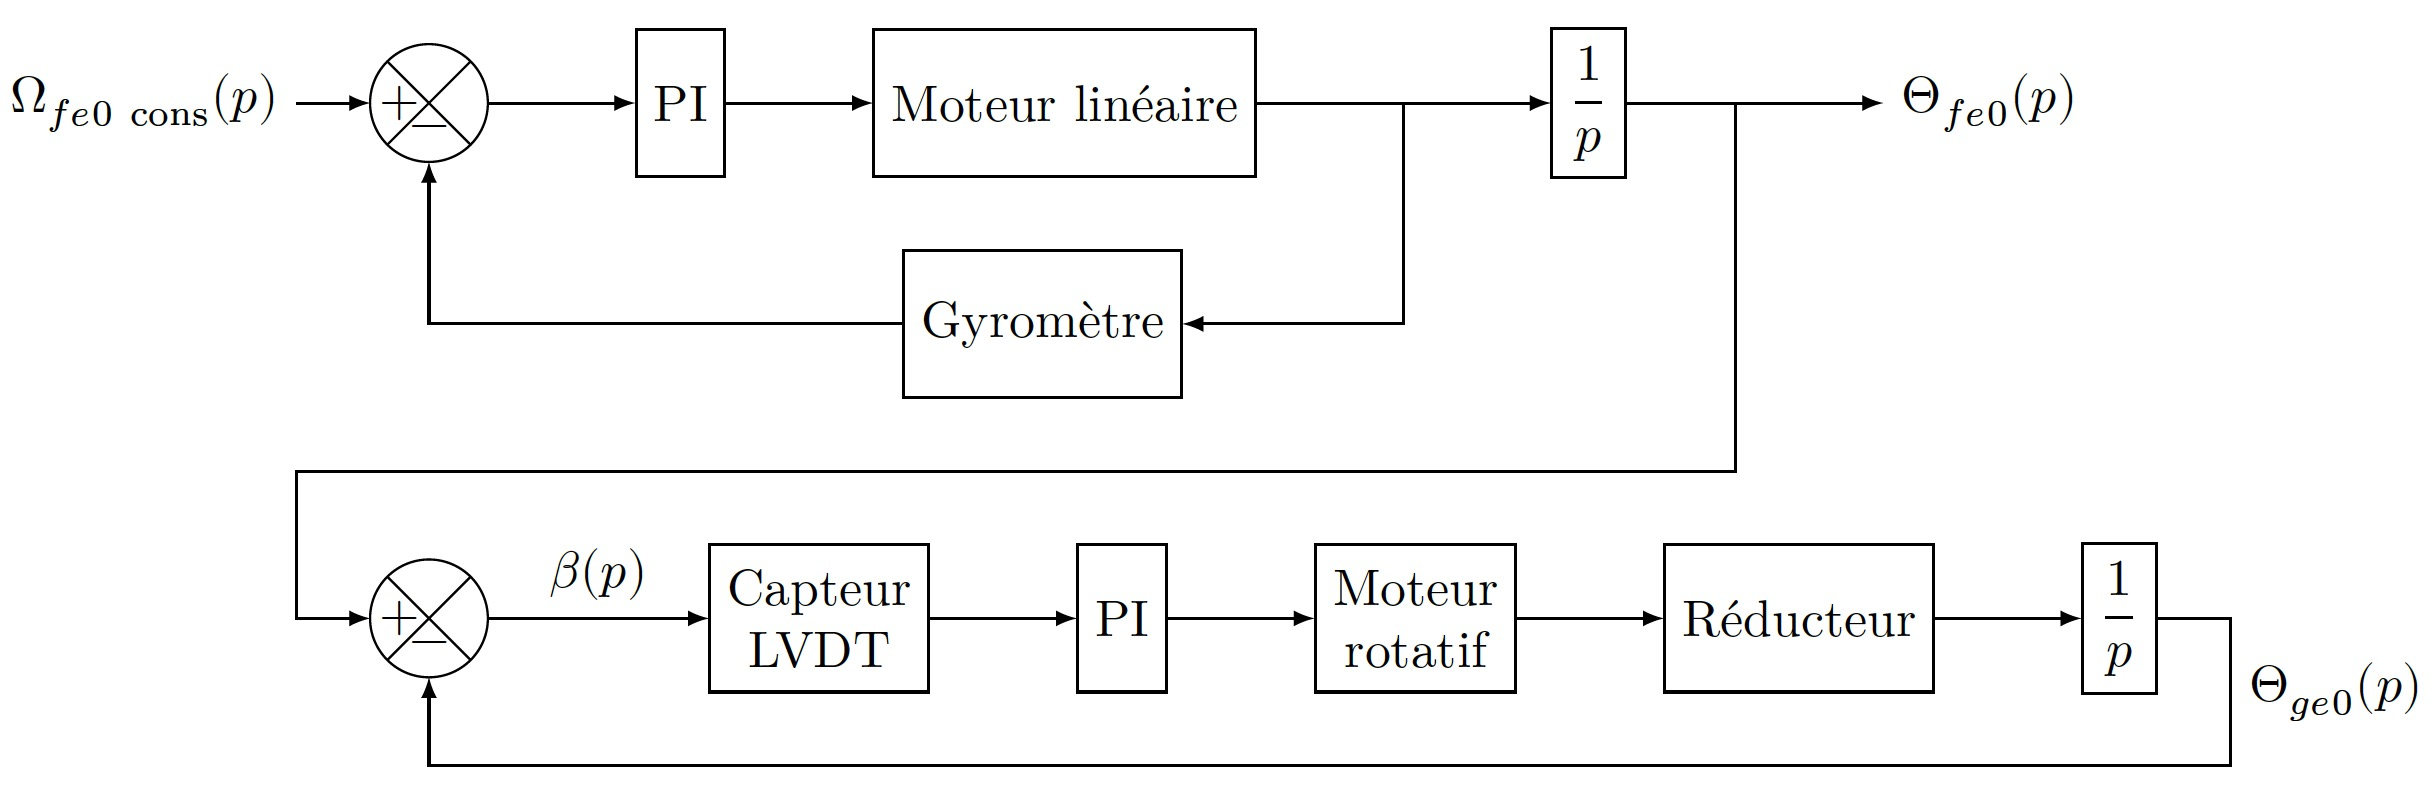
\includegraphics[width=1.0\textwidth]{figure18.jpg}
\caption{Modèle d'asservissement de l'axe motorisé d'élévation, PI représente un correcteur Proportionnel
Intégral \label{fig18}}
\end{center}
\end{figure}

La figure \ref{fig19} correspond à une mesure expérimentale du taux de rotation de la tête d'un pilote pour un mouvement
d'élévation de sa ligne de visée. Ce signal peut alors être utilisé comme signal de consigne envoyé à l'axe motorisé
d'élévation du FLIR.

\begin{figure}[!htb]
\begin{center}
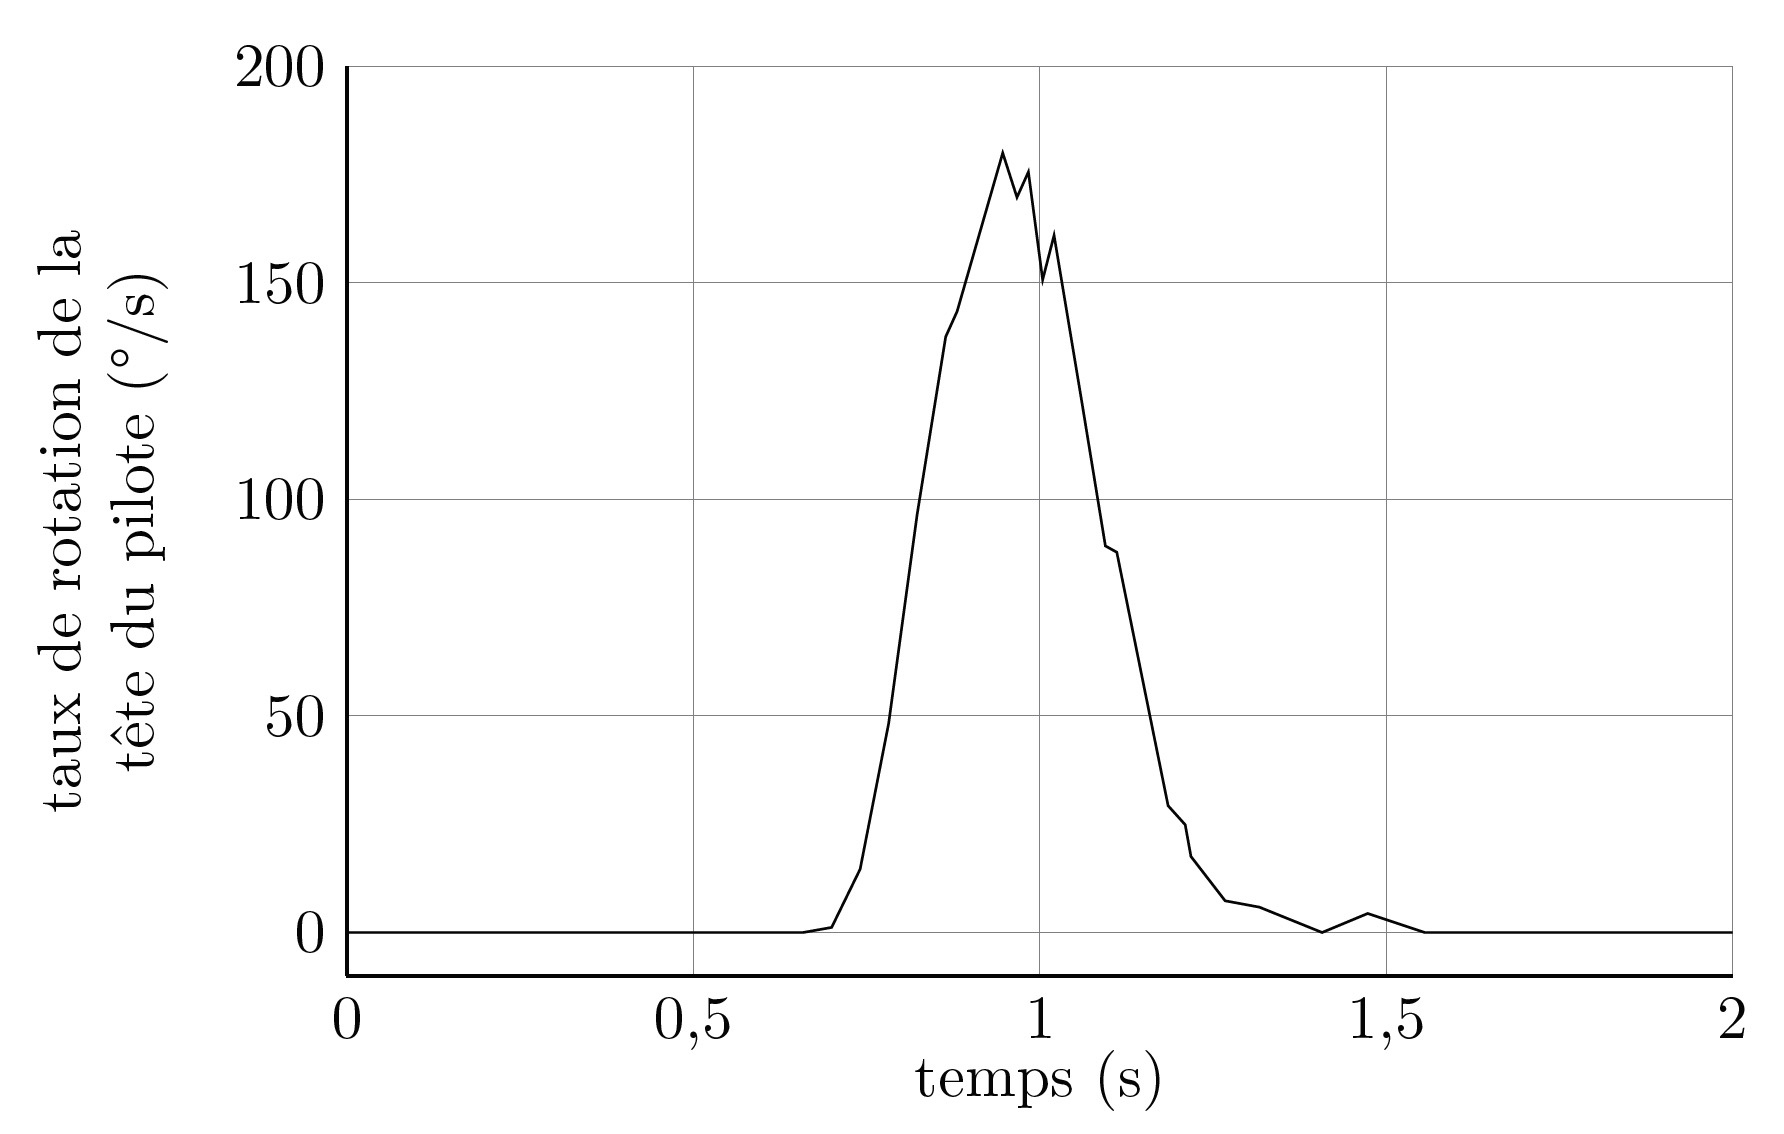
\includegraphics[width=1.0\textwidth]{figure19.jpg}
\caption{Mesure expérimentale du taux de rotation de la tête du
pilote (en degré par seconde) par rapport au référentiel galiléen, en
fonction du temps en seconde \label{fig19}}
\end{center}
\end{figure}

Pour simuler le modèle de l'axe motorisé d'élévation et comparer ses performances au cahier des charges du tableau \ref{tab2}, il est nécessaire de définir un signal de consigne $\omega_{fe0\text{ cons}}(t)$ composé des signaux canoniques utilisés
en automatique.

\question{À partir de la figure \ref{fig19} et en utilisant les signaux échelon et/ou rampe, proposer un modèle temporel
associé au signal de consigne $\omega_{fe0\text{ cons}}(t)$ exprimé en $rad\cdot s^{-1}$, sous la forme d'un tracé simple en fonction du temps en seconde. Tracer l'allure de $\theta_{fe0\text{ cons}}(t)$, exprimé en rad, qui correspond à l'évolution temporelle de la ligne de visée du pilote dans ce cas. Préciser les valeurs des points caractéristiques de ces deux courbes.}


\question{À partir des deux tracés précédents, indiquer quels critères du cahier des charges du tableau \ref{tab2} peuvent
être validés en utilisant ce signal de consigne dans la simulation du comportement de l'axe motorisé d'élévation
du FLIR. Après avoir dimensionné et implanté le correcteur proportionnel intégral (noté PI) au sein du modèle de l'étage
gros d'élévation (figure \ref{fig18}), on simule l'évolution de $\beta(t)=\theta_{fe0(t)}-\theta_{ge0}(t)$ pour le signal de consigne $\omega_{fe0\text{ cons}}(t)$ établi à partir de la mesure de la figure \ref{fig19}. Les résultats de simulation sont donnés sur la figure \ref{figB} du document réponse.}

\question{À partir de la figure \ref{figB} :}
\textit{
\begin{itemize}
\item vérifier si l'hypothèse $\vect{u}\approx \vect{z}_e$ reste valide ;
\item  pour chaque critère du cahier des charges du tableau \ref{tab2} et à l'aide de tracés sur le document réponse,
conclure sur l'aptitude du FLIR à respecter les performances du cahier des charges en comparant les valeurs
numériques mesurées sur les résultats de simulation à celles du tableau \ref{tab2}.
\end{itemize}
}